\usetikzlibrary{positioning, shapes, trees, graphs}

%rna, from 5' to 3':
% AUGCAAACUGGCACCCUCAU
% (((((...))(...))..))

\begin{center}
	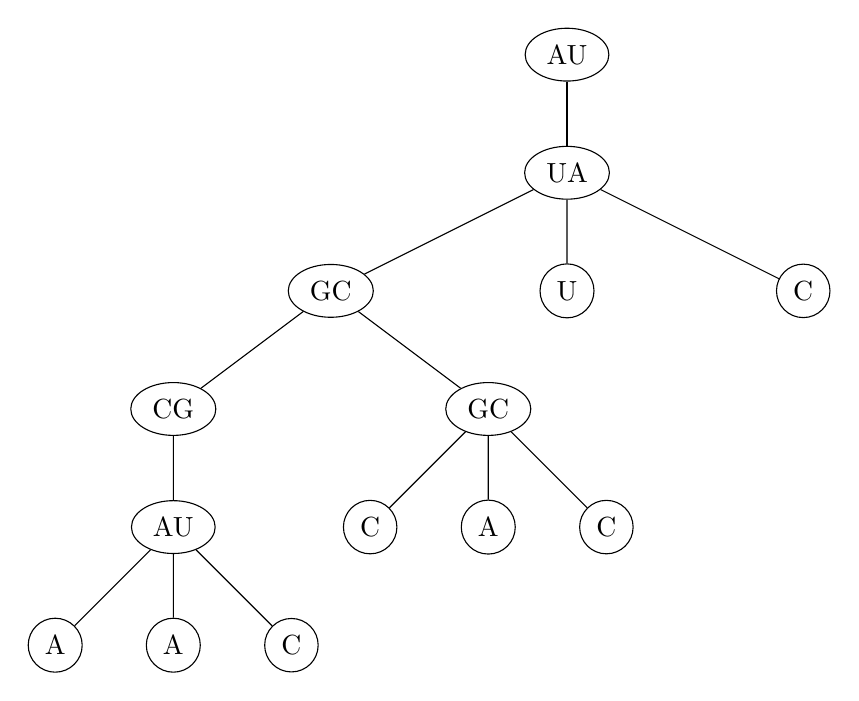
\begin{tikzpicture}[
			baseline,
			level distance = 1.5 cm,
			basepair/.style = {ellipse, draw, minimum height = 0.3 cm, minimum width = 0.7 cm},
			unpaired/.style = {circle, draw, minimum width = 0.3 cm},
			level 2/.style={sibling distance = 3 cm},
			level 3/.style={sibling distance = 4 cm},
			level 4/.style={sibling distance = 1.5 cm}
		]
		\node[basepair] {AU}
		child {
			node[basepair] {UA}
			child {
				node[basepair] {GC}
				child {
					node[basepair] {CG}
					child {
						node[basepair] {AU}
						child {
							node[unpaired] {A}
						}
						child {
							node[unpaired] {A}
						}
						child {
							node[unpaired] {C}
						}
					}
				}
				child {
					node[basepair] {GC}
					child {
						node[unpaired] {C}
					}
					child {
						node[unpaired] {A}
					}
					child {
						node[unpaired] {C}
					}
				}
			}
			child {
				node[unpaired] {U}
			}
			child {
				node[unpaired] {C}
			}
		}
		;
	\end{tikzpicture}
\end{center}

\begin{center}
	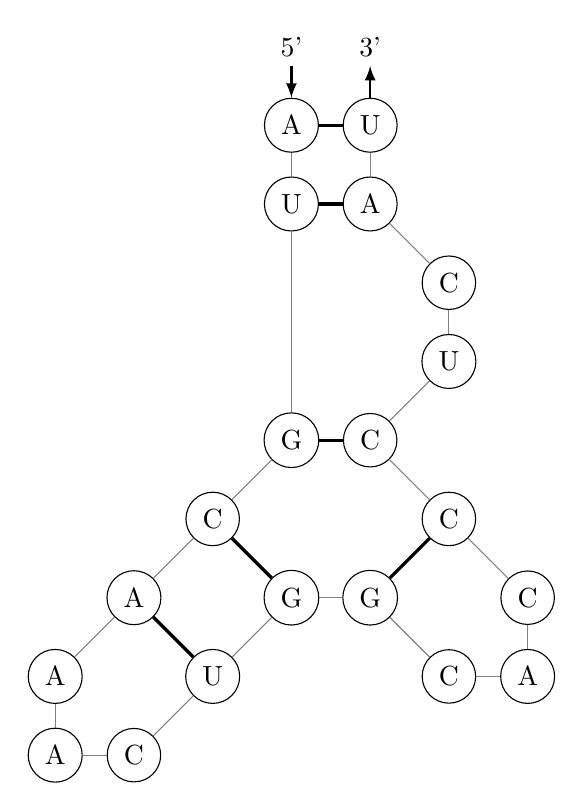
\begin{tikzpicture}[on grid, -latex,
			base/.style = {circle, draw, minimum width = 0.5 cm},
			ends/.style = {draw = none, fill = none}]

		%ends, 5' a 3'
		\node[ends] (5end) {5'};
		\node[ends] (3end) [right = of 5end] {3'};

		%stem
		\node[base] (StemLeft1) [below = of 5end] {A};
		\node[base] (StemRight1) [right = of StemLeft1] {U};
		\node[base] (StemLeft2) [below = of StemLeft1] {U};
		\node[base] (StemRight2) [right = of StemLeft2] {A};

		%bulge
		\node[base] (Bulge1) [below right = of StemRight2] {C};
		\node[base] (Bulge2) [below = of Bulge1] {U};

		%stem
		\node[base] (StemRight3) [below left = of Bulge2] {C};
		\node[base] (StemLeft3) [left = of StemRight3] {G};

		%left-branch
		\node[base] (LBranchLStem1) [below left = of StemLeft3] {C};
		\node[base] (LBranchRStem1) [below right = of LBranchLStem1] {G};
		\node[base] (LBranchLStem2) [below left = of LBranchLStem1] {A};
		\node[base] (LBranchRStem2) [below left = of LBranchRStem1] {U};

		%left-branch-hairpin
		\node[base] (LBranchHairpin1) [below left = of LBranchLStem2] {A};
		\node[base] (LBranchHairpin2) [below = of LBranchHairpin1] {A};
		\node[base] (LBranchHairpin3) [right = of LBranchHairpin2] {C};

		%right-branch
		\node[base] (RBranchRStem1) [below right = of StemRight3] {C};
		\node[base] (RBranchLStem1) [below left = of RBranchRStem1] {G};

		%right-branch-hairpin
		\node[base] (RBranchHairpin1) [below right = of RBranchLStem1] {C};
		\node[base] (RBranchHairpin2) [right = of RBranchHairpin1] {A};
		\node[base] (RBranchHairpin3) [below right = of RBranchRStem1] {C};

		\begin{scope}[-]
		%pair edges
			\path[very thick]
			(StemLeft1) edge (StemRight1)
			(StemLeft2) edge (StemRight2)
			(StemLeft3) edge (StemRight3)
			(LBranchLStem1) edge (LBranchRStem1)
			(LBranchLStem2) edge (LBranchRStem2)
			(RBranchLStem1) edge (RBranchRStem1)
			;
		%lines around molecule
			\path[color = gray]
			(StemLeft1) edge (StemLeft2)
			(StemLeft2) edge (StemLeft3)
			(StemLeft3) edge (LBranchLStem1)
			(LBranchLStem1) edge (LBranchLStem2)
			(LBranchLStem2) edge (LBranchHairpin1)
			(LBranchHairpin1) edge (LBranchHairpin2)
			(LBranchHairpin2) edge (LBranchHairpin3)
			(LBranchHairpin3) edge (LBranchRStem2)
			(LBranchRStem2) edge (LBranchRStem1)
			(LBranchRStem1) edge (RBranchLStem1)
			(RBranchLStem1) edge (RBranchHairpin1)
			(RBranchHairpin1) edge (RBranchHairpin2)
			(RBranchHairpin2) edge (RBranchHairpin3)
			(RBranchHairpin3) edge (RBranchRStem1)
			(RBranchRStem1) edge (StemRight3)
			(StemRight3) edge (Bulge2)
			(Bulge2) edge (Bulge1)
			(Bulge1) edge (StemRight2)
			(StemRight2) edge (StemRight1)
			;
		\end{scope}

		\begin{scope}
			% edges to ends
			\path[thick]
			(5end) edge (StemLeft1)
			(StemRight1) edge (3end)
			;
		\end{scope}
	\end{tikzpicture}
\end{center}

